\documentclass{standalone}
\usepackage{tikz}
\begin{document}
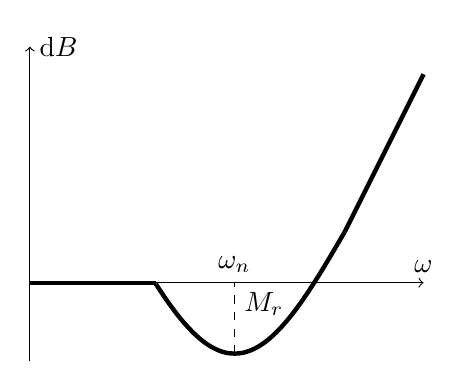
\begin{tikzpicture}[scale=2]
    \draw[->](-1,0)--(1.5,0)node[above]{$\omega$};
    \draw[->](-1,-0.5)--(-1,1.5)node[right]{$\mathrm{d} B$};

    \draw[-,ultra thick](-1,0)--(-0.2,0);
    \draw[-, ultra thick]plot[smooth, domain=-0.2:1](\x,{1.55-2*e^-(\x-0.3)^2});

    \draw[dashed](0.3,-0.45)--(0.3,0)node[above]{$\omega_n$}node[below right]{$M_r$};
    \draw[-,ultra thick](1,0.324)--(1.5,1.324);
\end{tikzpicture}
\end{document}